\documentclass{beamer}
\usetheme{ensam}
\usepackage{pgfplots}
\usepackage{subcaption}
\usepackage{acronym}
\usepackage{tikz}
\usetikzlibrary{calc}
\usepackage{amsmath}
\usepackage{multirow}
\usepackage {algorithmic}
\usepackage{booktabs}
\usepackage{algorithm}
\usepackage{eqparbox}
\usepackage[font=scriptsize]{caption}
\usetikzlibrary{bayesnet,positioning,calc}
\tikzstyle{obs} = [latent,fill=lightBlue]
\tikzstyle{default}=[draw=sexyRed,thick,rounded corners,text width=0.5in,font=\scriptsize,align=center]
\usepgfplotslibrary{colorbrewer}
\definecolor{ForestGreen}{RGB}{34,139,34}
\newcommand{\comment}[1]{\textcolor{ForestGreen}{#1}}
%algorithmic comment
\renewcommand\algorithmiccomment[1]{%
  \hfill\comment{\#\scriptsize\eqparbox{COMMENT}{#1}}%
}
\renewcommand{\algorithmicrequire}{\textbf{Input:}}
\renewcommand{\algorithmicensure}{\textbf{Output:}}
\title{Intélligence artificielle}
\author{\underline{A.Belcaid}}
\institute{Ecole Nationale des Sciences Appliquées Fès} 
\date{18 Mars 2019}

%tikz bayesian theme
\usetikzlibrary{bayesnet,positioning,calc}
\tikzstyle{obs} = [latent,fill=lightBlue]
\tikzstyle{default}=[draw=sexyRed,thick,rounded corners,text width=0.5in,font=\scriptsize,align=center]
\DeclareMathOperator{\argmin}{argmin}

\pgfplotsset{every tick label/.append style={font=\tiny}}



%acronyms
\acrodef{AI}{Artificial Intelligence}


% add bibliography
\usepackage[style=authoryear]{biblatex}
\renewcommand*{\nameyeardelim}{\addcomma\addspace}
% \addbibresource{bibliography}

\begin{document}
\maketitle



\begin{frame}[t]{Présentation du cours}
  \begin{figure}
    \centering
  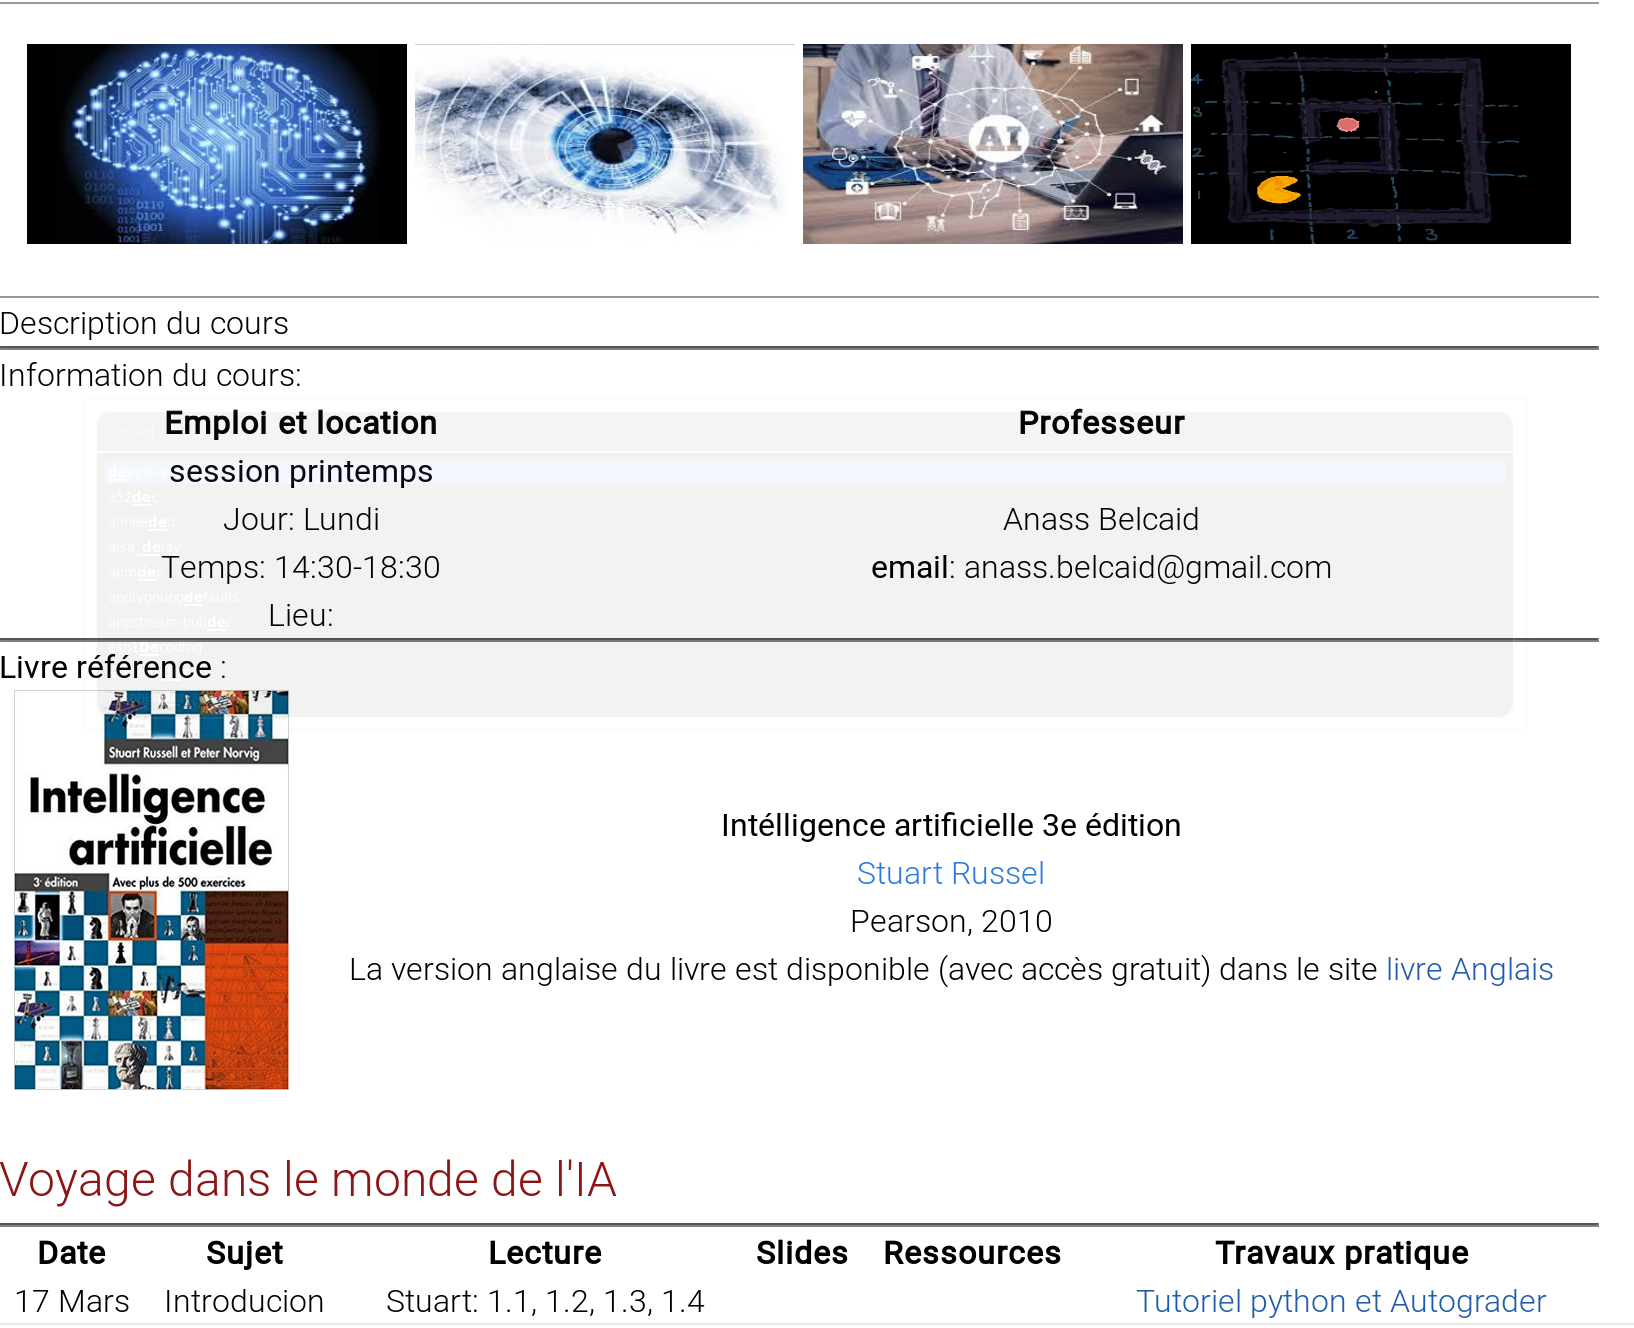
\includegraphics[width=\textwidth,height=7cm]{./images/preview_site.png}  
  \caption*{https://intelligenceartificielensaf.github.io/}
\end{figure}
\end{frame}

\begin{frame}[<+->]{Information du cours}
  \begin{itemize}
    \item \alert{Prérequis}

      \begin{itemize}
        
        \item {\scriptsize \textbf{Mathématiques} ( probablités, algèbre, théorie de
          graphes)}
        \item {\scriptsize\textbf{Fondement de programmation} ( Structure de données, paradigmes de
          programmation ( récurrence, programmation dynamique).}
        \item {\scriptsize \textbf{Python} : bases des langages voir tutorial }
      \end{itemize}
    \item \alert{Note finale}
      \begin{table}[htpb]
        \centering
        \begin{tabular}{cc}
          \toprule
          \structure{\textbf{Element}} & \structure{\textbf{pourcentage}}\\
          \midrule
        \pause
          
          {\scriptsize Participation, TD}   & {\scriptsize $5\%$}\\\pause
          {\scriptsize Test(midterm)}   & {\scriptsize $20\%$}\\\pause
          {\scriptsize Examen}   & {\scriptsize $50\%$}\\\pause
          {\scriptsize Projets}   & {\scriptsize $25\%$}\\
          {\scriptsize Notes cours}   & {\scriptsize $??\%$}\\
          \bottomrule
        \end{tabular}
      \end{table}
  \end{itemize}
\end{frame}

\begin{frame}[t]{Livre de référence}
  \begin{figure}[htpb]
    \centering
    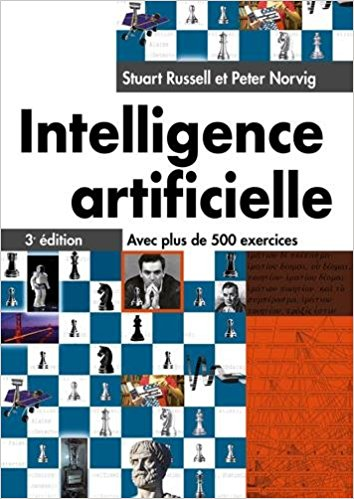
\includegraphics[width=0.3\linewidth,height=5cm]{./images/book_cover.jpg}
    \caption*{ \href{https://www.amazon.fr/dp/2744074551/ref=pe_3044141_189395771_TE_3p_dp_1}{Intélligence artificielle 3e édition} }
    \label{fig:./images/book_cover}
  \end{figure} 

\small Version anglaise du livre est \alert{libre} dans le site
{\scriptsize
\structure{\href{http://aima.cs.berkeley.edu/}{http://aima.cs.berkeley.edu/}}}
\end{frame}

\begin{frame}{Table de matieres}
  \begin{columns}
    \begin{column}{0.5\textwidth}
      {\scriptsize
      \begin{enumerate}
        \item Définition de \ac{AI}\\

        \item Fondements de \ac{AI}\\

        \item Histoire de l'\ac{AI}\\

        \item Etat de l'art\\

        \item Thèmes traités dans ce cours.
      \end{enumerate}
    }
    \end{column}
    \begin{column}{0.5\textwidth}
    \centering
    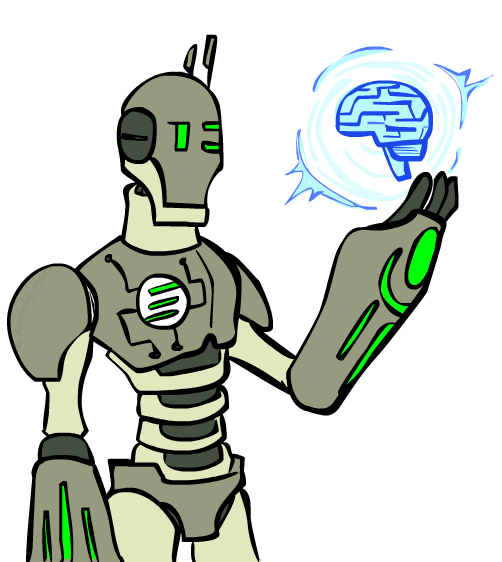
\includegraphics[width=0.8\textwidth]{./images/robot_contents.png}
    \end{column}
  \end{columns}
\end{frame}

%%%%%%%%%%%%%%%%%%%%%%%%
%  Définition de L'IA  %
%%%%%%%%%%%%%%%%%%%%%%%%
\section{Définition de l'AI}%
\label{sec:definition_de_l_ai}

\begin{frame}[t]{Intelligence artificielle: Vue future}
  
  \begin{tabular}{ccc}
    \centering
    \multirow{2}{*}{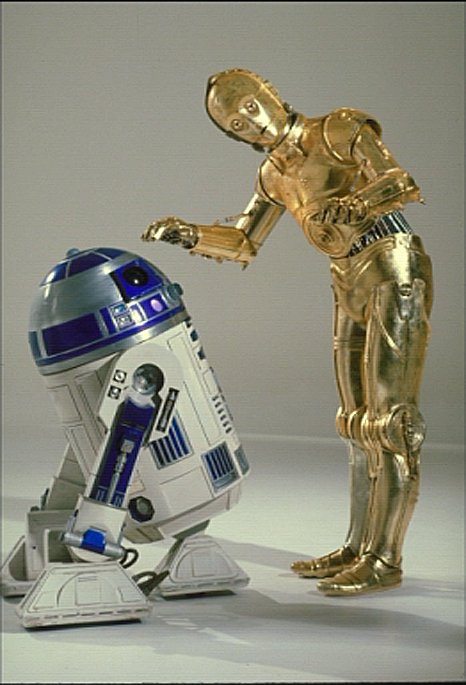
\includegraphics[width=3cm,height=6cm]{./images/movie_1.png}} &
    \pause
    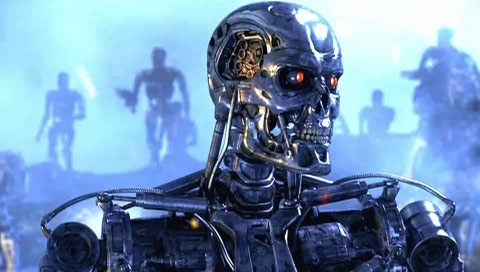
\includegraphics[width=3cm,height=3cm]{./images/movie_2.png} &\pause
    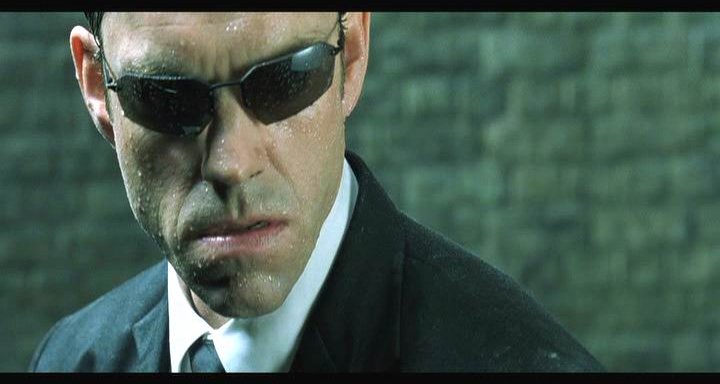
\includegraphics[width=3cm,height=3cm]{./images/movie_3.png}\\\pause
    &
    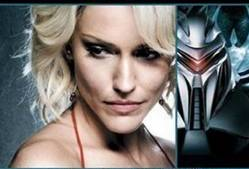
\includegraphics[width=3cm,height=3cm]{./images/movie_4.png}& \pause
    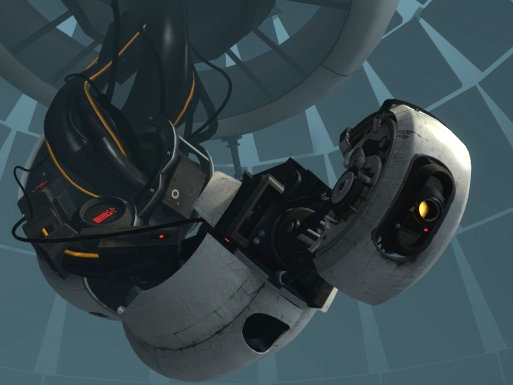
\includegraphics[width=3cm,height=3cm]{./images/movie_5.png}\\
  \end{tabular}
\end{frame}


%%%%%%%%%%%%%%%%%%%%%%%%
%  Définition de l'IA  %
%%%%%%%%%%%%%%%%%%%%%%%%

\begin{frame}[t]{Définition de l'AI}
  
\centering
\begin{tabular}{m{2cm}m{4cm}m{4cm}}
  & \textbf{Humain} & \textbf{Rationnel} \\

  \structure{\textbf{Penser}}  &
  \only<1->{ 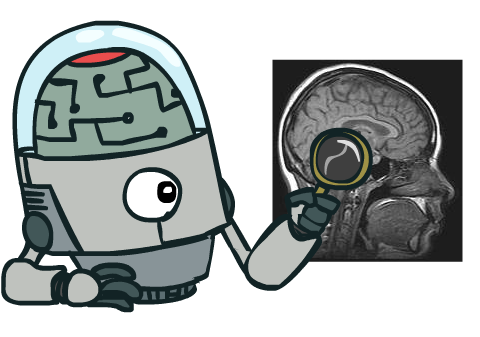
\includegraphics[width=3cm,height=3cm]{./images/think_humain.png}}
  &
  \only<3->{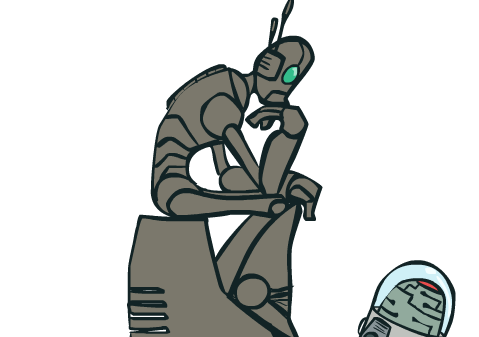
\includegraphics[width=3cm,height=3cm]{./images/think_rational.png}}
    \\
  \textbf{\alert{Agir}} &
                        
  \only<2->{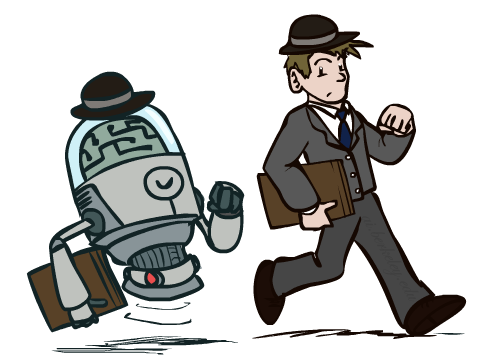
\includegraphics[width=3cm,height=3cm]{./images/act_humain.png}}
                        & 

                        \only<4>{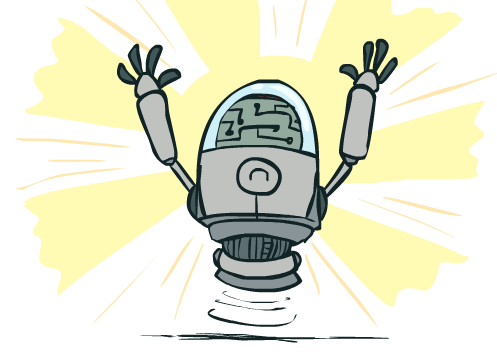
\includegraphics[width=3cm,height=3cm]{./images/act_rational.png}}
\end{tabular}
\end{frame}

%%%%%%%%%%%%%%%%%%%%%%%%%
%  Agir rationnellemet  %
%%%%%%%%%%%%%%%%%%%%%%%%%

\begin{frame}[<+->]{Action rationnelle}
  \begin{itemize}
    \item Achever et réaliser les objectifs définis.
    \item Se concentre uniquement sur la \alert{\textbf{décision prise}} et non pas sur le
      \textbf{processus} de décision.
    \item Les objectifs doivent être exprimés en terme d'une fonction
      \textbf{\alert{Utilité}} du résultat.
\end{itemize}

\begin{block}{title}
  
  Être rationnel c'est  optimiser (\textbf{maximiser}) sa propre fonction
  d'\textbf{utilité}
\end{block}
\end{frame}

\begin{frame}[t]

  \huge{\textbf{Maximiser l'espérance de sa fonction d'utilité}}
  \begin{figure}[htpb]
    \centering
    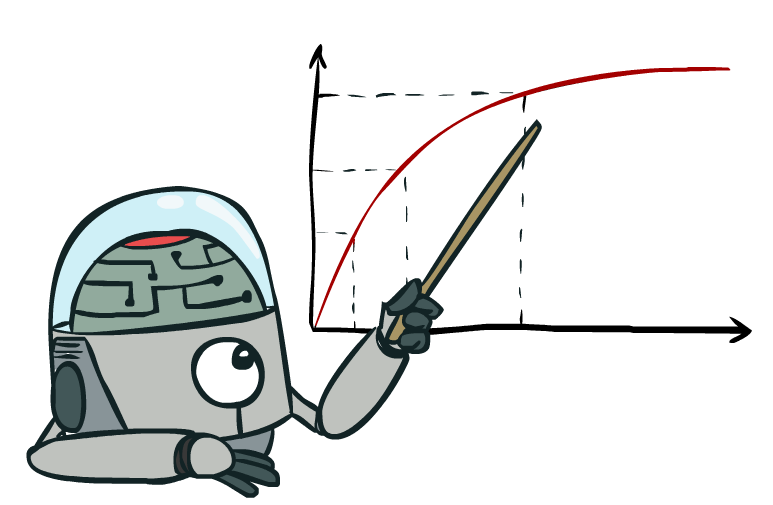
\includegraphics[width=0.8\linewidth]{./images/maximize_expected_utility.png}
  \end{figure}
\end{frame}

%%%%%%%%%%%%%%%%%%%%%%%%%%%%%%%%%%
%  Vue simple du cerveau humain  %
%%%%%%%%%%%%%%%%%%%%%%%%%%%%%%%%%%

\begin{frame}[t]{Vue simple du cerveau humain}
  \begin{columns}
    \begin{column}{0.5\textwidth}
      {\small
        \begin{itemize}
           
          \item Le cerveau humain excelle dans la prise des décisions rationnels 
          \item Le cerveau n'est pas modulaire comme les logiciels, et donc il
            est très difficile
    inverser le processus de pensée.
  \item<2-> Cerveaux pour l'intelligence sont des ails pour voler.
  \item<2-> Leçons apprises du cerveau: 
    \begin{itemize}
      \scriptsize
    \item \alert{\textbf{Mémorisation}}: apprendre des expériences
    \item \alert{\textbf{Simulation}}:  apprendre à  simuler une chaine d'actions
    \end{itemize}
        \end{itemize}
      }
    \end{column}
    \begin{column}{0.5\textwidth}
      \only<1>{ 
      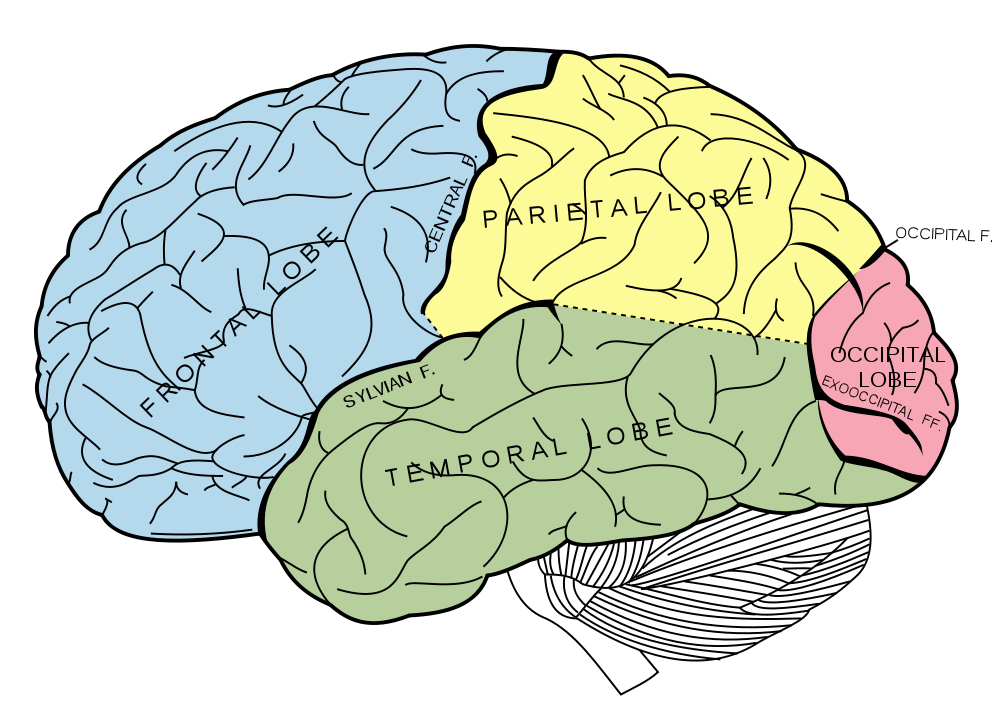
\includegraphics[width=1\linewidth,height=4cm]{./images/humain_brain.png}}
      \only<2>{ 
      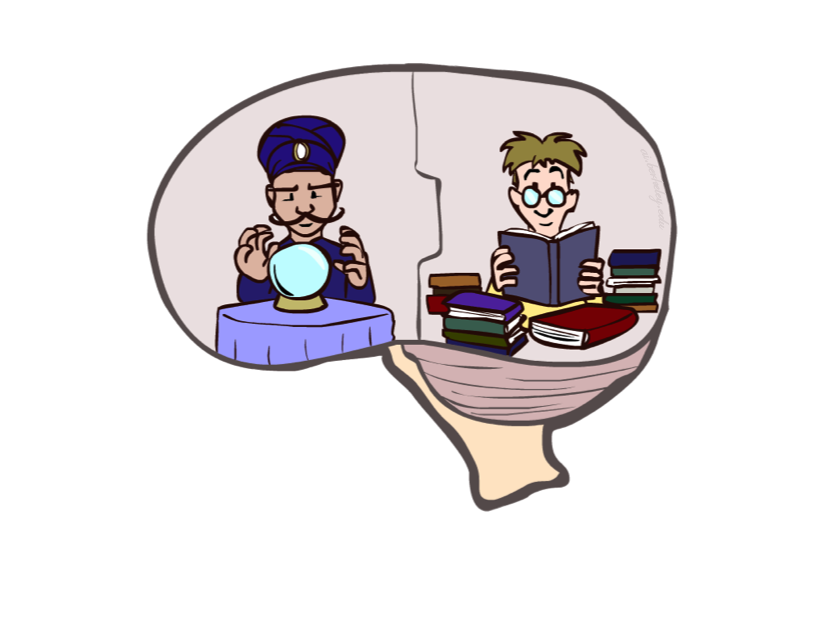
\includegraphics[width=1\linewidth,height=4cm]{./images/humain_brain_essential.png}}
    \end{column}
  \end{columns}
\end{frame}


\section{Histoire de l'AI}%
\label{sec:histoire_de_l_ai}

\begin{frame}[<+->]{Histoire de l'AI}
 \begin{columns}

   \begin{column}{0.3\textwidth}
\centering
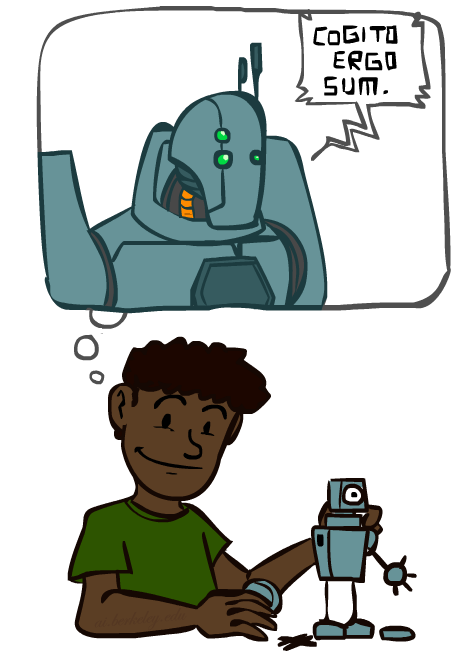
\includegraphics[width=1\linewidth,height=8cm]{./images/dream_ai.png}
   \end{column}
   \begin{column}{0.7\textwidth}
     {\scriptsize
    \begin{description}
      \item[\scriptsize Gestation de l'AI (1943-1955)]: 
        \begin{itemize}
          \item McCulloch, Walter Pitts (1943): Circuit booléen par réseaux de
            neurones.
          \item Alin Turing: Machinerie de l'intelligence.
      \end{itemize}
      \item[\scriptsize Naissance AI (1956)]:
        \begin{itemize}
          \item Programme Dames (Samuel) (1950)
          \item Worshop Darthmouth (1965)
          \item Programme de raisonnement logique: Robinson (1965)
        \end{itemize}

      \item[\scriptsize Systèmes de gestion de connaissance (1970-1990)]: 
        \begin{itemize}
          \item Systèmes basées sur la connaissance (1969-1979)
          \item Explosion des systèmes experts (1980-1988)
        \end{itemize}
      \item[\scriptsize Approche probabiliste(1990-présent)]:
        \begin{itemize}
          \item Modélisation et décision avec incertitude.
          \item Agents intelligents
        \end{itemize}
    \end{description} 
  }
   \end{column}
 \end{columns}
\end{frame}

\section{État de l'art}%
\label{sec:etat_de_l_art}
\newcommand{\cmark}{\ding{51}}%
\newcommand{\xmark}{\ding{55}}%
\begin{frame}[<+->]{Possibilités actuelles de l'AI}
  
  \begin{itemize}

    \item[$\square$]\structure<2->{ \textbf{Jouer pinball}}
  \item[$\square$] \structure<3->{\textbf{Jouter à questions pour un champion}}
  \item[$\square$]\alert<4->{\textbf{Conduire une voiture}}
  \item[$\square$]\structure<5->{\textbf{ Acheter une liste dans le Web}}
  \item[$\square$]\alert<6->{\textbf{ Acheter une liste dans un supermarché}}
  \item[$\square$]\structure<7->{ \textbf{Découvrir et démontrer un théorème
    mathématique}}
  \item[$\square$]\structure<8->{\textbf{ Discuter avec une personne}}
  \item[$\square$]\alert<9->{\textbf{Chirurgie médicale}}
\item[$\square$]\structure<10->{\textbf{ Faire le ménage }}
\item[$\square$]\structure<11->{\textbf{ Traduire des langes en temps réel}}
\item[$\square$]\structure<12->{\textbf{ Annoter des images}}
  \end{itemize}
\end{frame}


%%%%%%%%%%%%%%%%%%%%%%%%%%%%%%%%
%  Natural language processus  %
%%%%%%%%%%%%%%%%%%%%%%%%%%%%%%%%

\begin{frame}[t]{Langage Naturel}
     
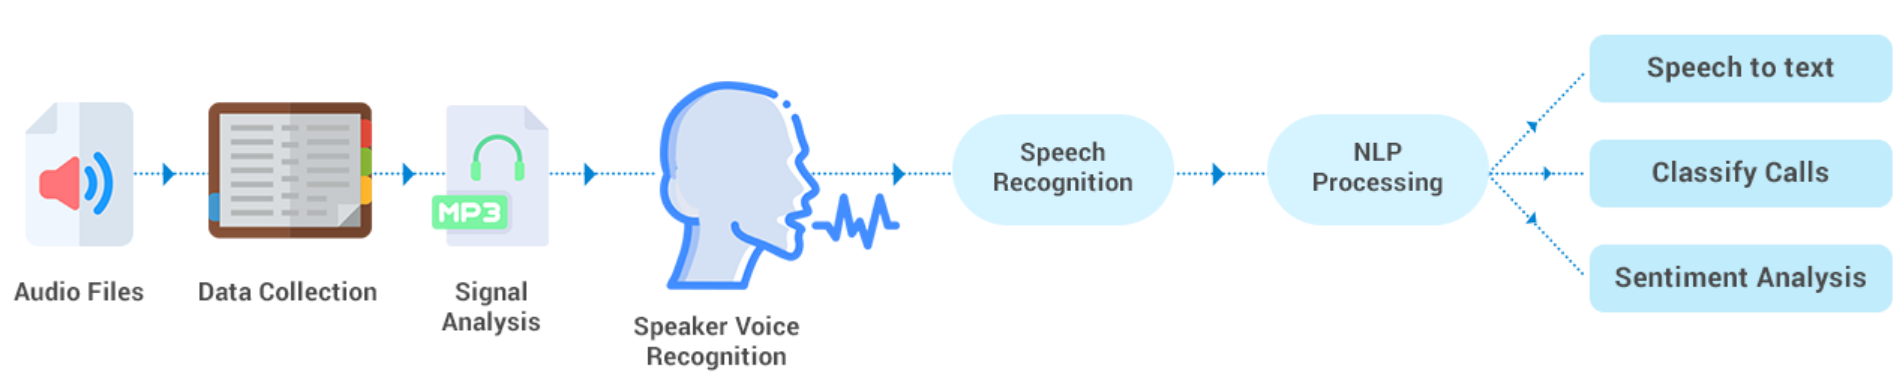
\includegraphics[width=0.9\linewidth,height=4cm]{./images/speech_recognition_1.png}

\begin{itemize}
  \item Synthèse du texte a partir du discours.
  \item Translation du discours.
  \item Classification des sentiments
  \item Demo
    \href{https://text-to-speech-demo.ng.bluemix.net/}{\alert{Speech
    synthesis}}
\end{itemize}
\end{frame}
%computer visiono

\begin{frame}{computer Vision}
  \begin{tabular}{cc}
    \centering
    \only<1->{Edge to image} &  \only<2->{structure to image}\\
    \only<1->{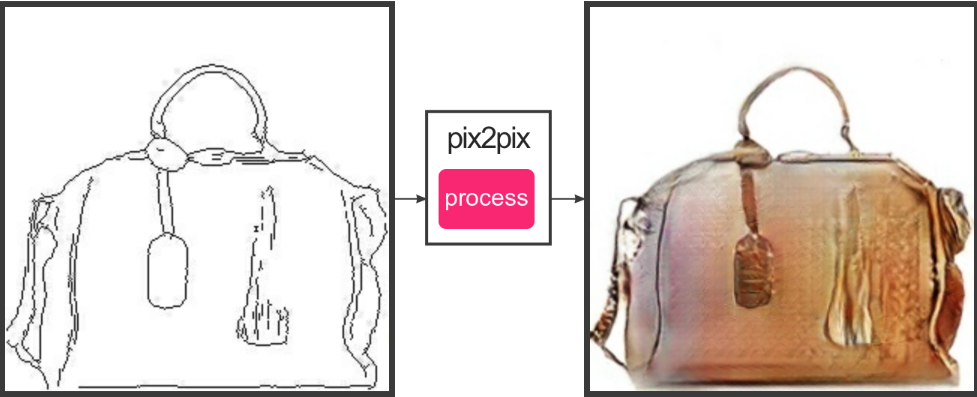
\includegraphics[width=0.4\linewidth,height=3cm]{./images/edge_to_image.png}}
    &
    \only<2->{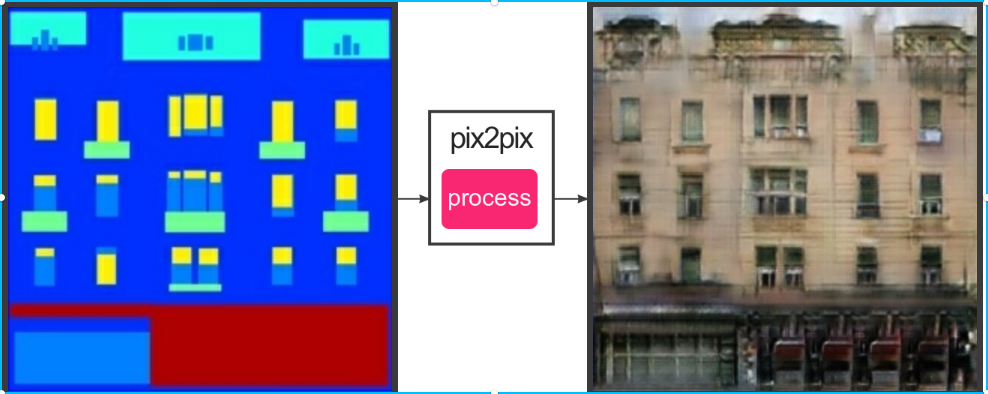
\includegraphics[width=0.4\linewidth,height=3cm]{./images/structure_to_image.png}}
    \\
    \only<3->{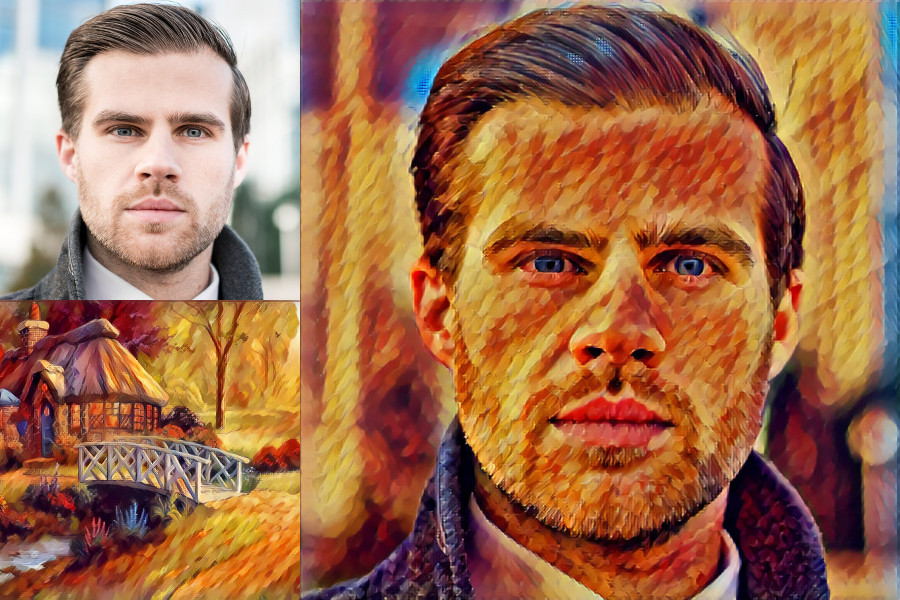
\includegraphics[width=0.4\linewidth,height=3cm]{./images/deep_dream.jpg}}
    & 
    \only<4->{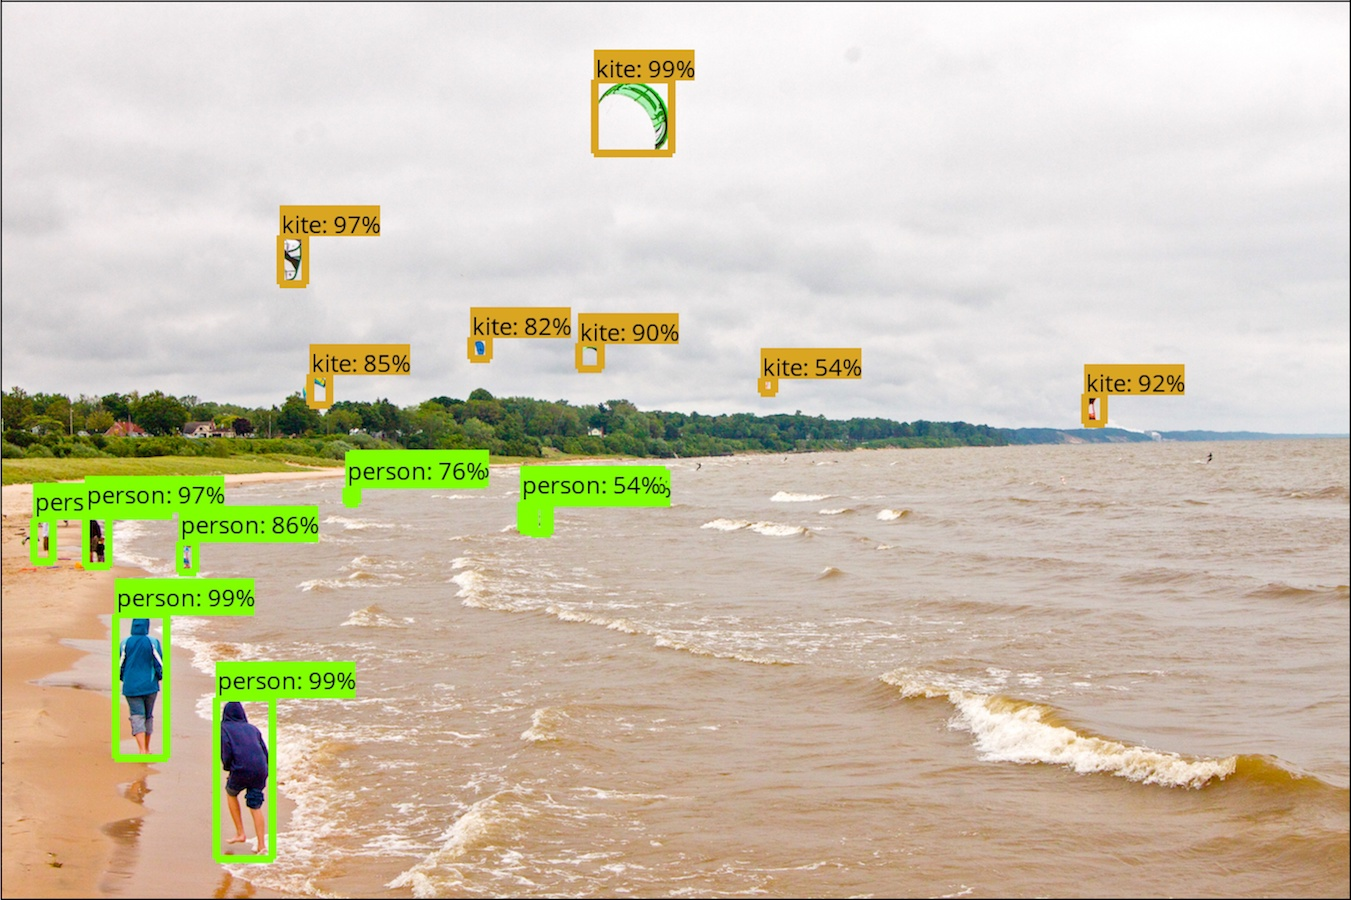
\includegraphics[width=0.4\linewidth,height=3cm]{./images/tensor_object_detection.jpg}}
    \\
    \only<3->{Deep Dream} & \only<4>{Object detection}\\
  \end{tabular}
\end{frame}

%%%%%%%%%%%%%%%%
%  Robotiques  %
%%%%%%%%%%%%%%%%

\begin{frame}[t]{Robotique}
  \begin{columns}
    \begin{column}{0.5\textwidth}
      \begin{tabular}{c}
    \only<1->{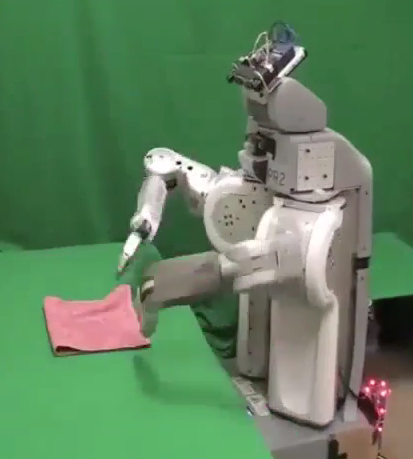
\includegraphics[width=0.9\linewidth,height=3cm]{./images/landery.png}}\\

    \only<2->{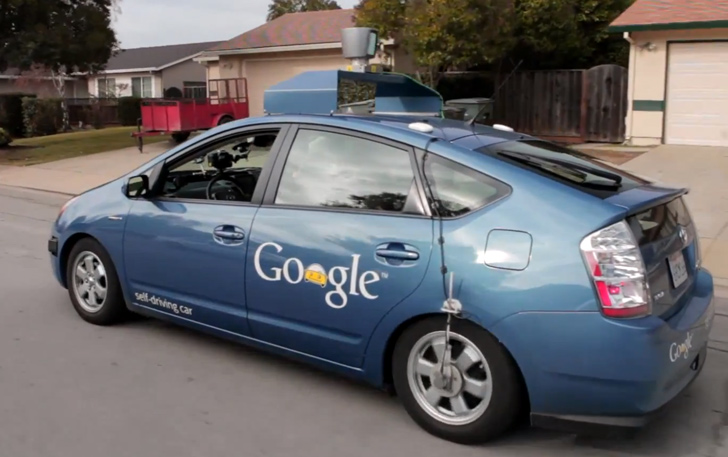
\includegraphics[width=0.9\linewidth,height=3cm]{./images/google_car.png}}
      \end{tabular}
    \end{column}
    \begin{column}{0.5\textwidth}
      
    \only<3->{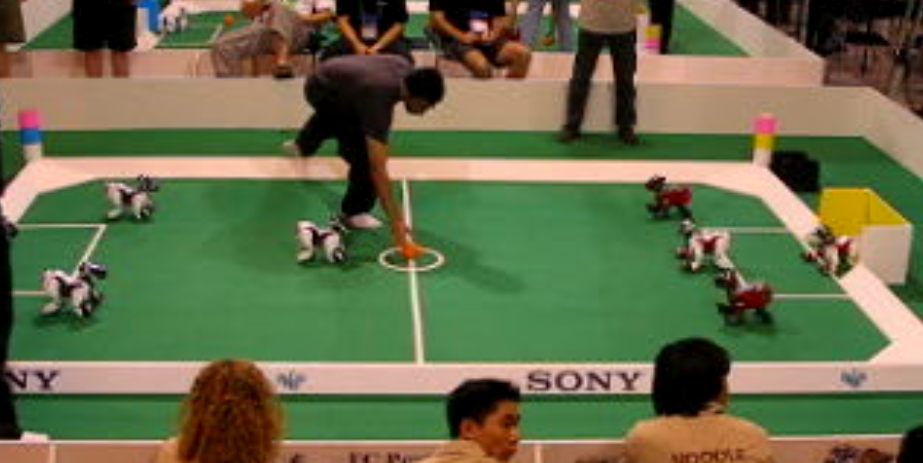
\includegraphics[width=0.9\linewidth,height=6cm]{./images/robots_football.png}}
    \end{column}
  \end{columns}
  \centering
  \alert{Demo}
\end{frame}


%%%%%%%%%%
%  Jeux  %
%%%%%%%%%%
\begin{frame}[t]{Jeux}
  \begin{columns}
    \begin{column}{0.5\textwidth}
      \scriptsize{ 
      \begin{itemize}
        \item 1996  Kasparov domine \textbf{DeepBlue} 
        \item 1997 \textbf{DeepBlue} bat le champion du monde 
        \item Traitement de plus de 200 positions par second.
        \item 2017 \textbf{AlphaGo} domine le champion du monde en \alert{GO}  
      \end{itemize}
    }
    \end{column}
    \begin{column}{0.5\textwidth}
      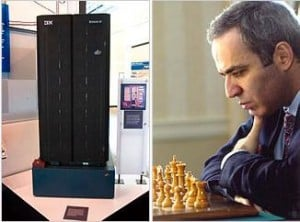
\includegraphics[width=0.9\textwidth,
      height=4cm]{./images/deepBlue_kasparov.jpg} 
      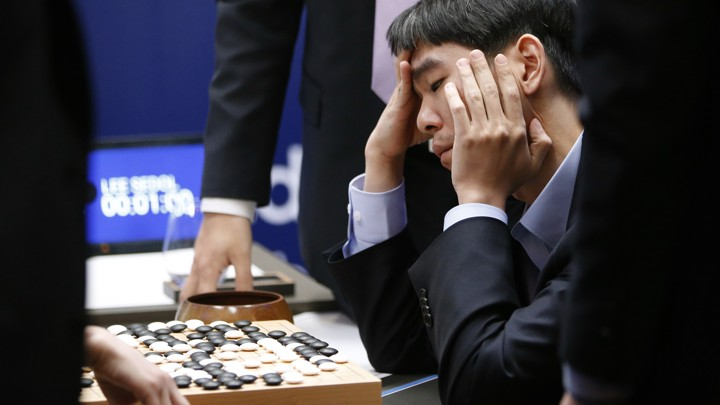
\includegraphics[width=0.9\textwidth,
    height=4cm]{./images/alphago-2.jpg} 
    \end{column}
  \end{columns}
\end{frame}

%%%%%%%%%%%%%%%%%%%%%%%
%  Prise de décision  %
%%%%%%%%%%%%%%%%%%%%%%%

\begin{frame}[t]{Prise de décision}
\begin{columns}
  \begin{column}{0.5\textwidth}
    \begin{itemize}
      \item Filtre de Spam 
      \item Ordonnancement des vols.
      \item Logistique
      \item Diagnostique médical.
      \item Systèmes de recommandation.
      \item $\ldots.$
    \end{itemize} 
  \end{column}
  \begin{column}{0.5\textwidth}
    \only<1->{
\includegraphics[width=0.9\textwidth,
      height=4cm]{./images/spam_filtering.png}  }
    \only<1->{
\includegraphics[width=0.9\textwidth,
      height=4cm]{./images/medical_diagnostic.png} }
  \end{column}
\end{columns}  
\end{frame}


\begin{frame}[t]{Agents rationnels}
  \only<1->{
  \begin{columns}
    \begin{column}{0.5\textwidth}
     \begin{block}{}
       \small
       Un \textbf{agent}(\emph{agere} :faire) est une entité qui
       \textbf{\structure{pércoit}} son monde extérieur et
       \alert{\textbf{agit}}
     \end{block} 
     \pause
     \begin{block}{}
       \small
       Un \alert{\textbf{agent rationnel}} doit  choisir l'\textbf{action} qui maximise
       (\emph{l'espérance}) de sa fonction \textbf{d'utilité} 
     \end{block} 
    \end{column}
    \begin{column}{0.5\textwidth}
      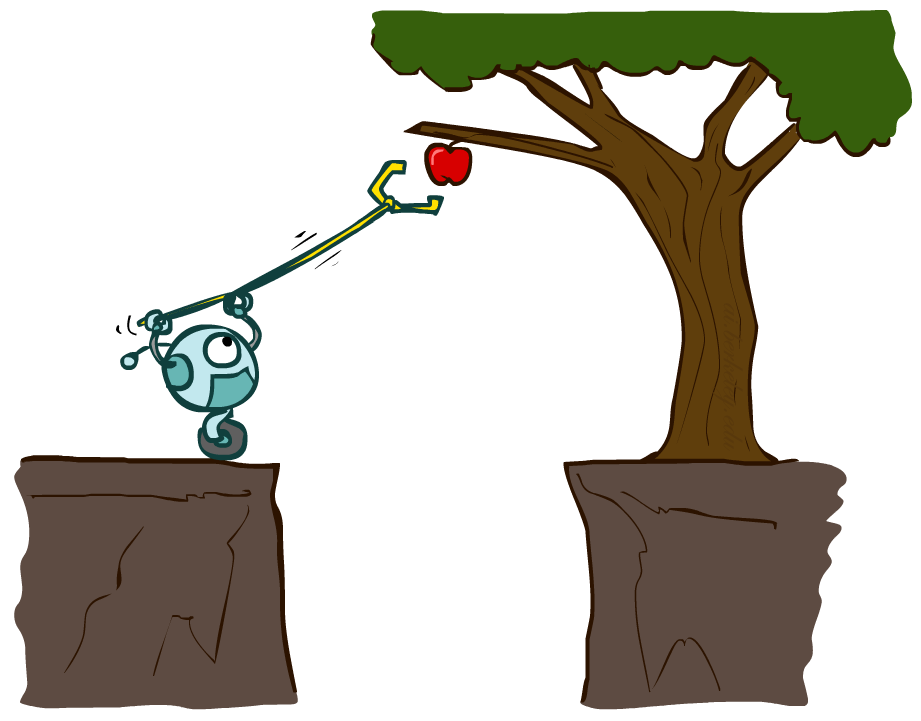
\includegraphics[width=0.9\textwidth,height=4cm]{./images/agent_perception.png}
    \end{column}
  \end{columns}
}

\only<2->
{

  \begin{columns}
    \begin{column}{0.5\textwidth}
     \begin{block}{}
       \scriptsize
       Les caractéristiques de l'\textbf{observabilité} de
       \textbf{l'environnement} et
       l'\alert{\textbf{espace des actions}} décrivent les techniques a adoptés
       pour un agent.
     \end{block} 
    \end{column}
    \begin{column}{0.5\textwidth}
      \centering
      \begin{tikzpicture}[yscale=0.7,xscale=0.8]
        \node (sensors) at (0,1) {\scriptsize Senseurs};
        \node [draw, rounded corners,minimum width=0.5cm](actions) at (0,0)
          {\scriptsize \textbf{?}};
        \node (actuators) at (0,-1) {\scriptsize Actionneurs};

        \node[rounded corners, fill=lightBlue, rotate =-90,opacity=0.6,minimum
          height=1cm] (env) at (3,0) {Environnement};
        
        \path[draw,->,thick](actuators)--(2.5,-1);
        \path[draw,->,thick](2.5,1)--(sensors);
        \path[draw,thick](sensors)--(actions)--(actuators);

        %hope
        \node[rounded corners, fit
          =(sensors)(actuators),draw,label=left:Agent,fill = sexyRed,opacity=0.3](agent) {};
      \end{tikzpicture}
    \end{column}
  \end{columns}

}
\end{frame}


\begin{frame}[t]{L'agent Pacman}
  
\begin{figure}[htpb]
  \centering
  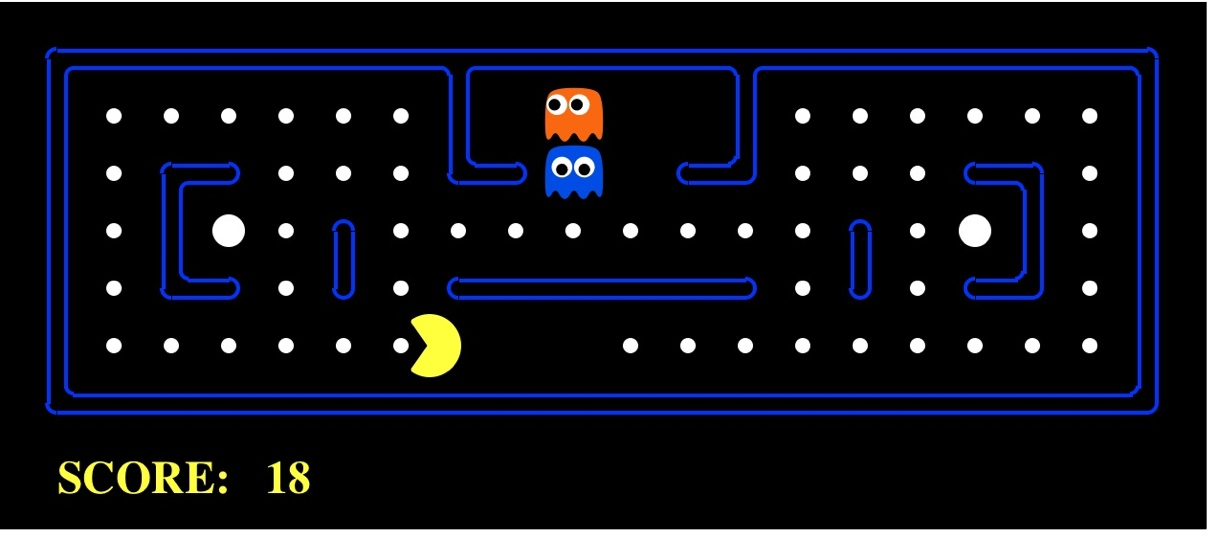
\includegraphics[width=0.8\linewidth,height=5cm]{./images/pacman_as_agent.png}
  \caption*{Agent Pacman}
  \label{fig:}
\end{figure}
\end{frame}


\begin{frame}[<+->]{Thématiques du cours}
 \begin{description}
 \item[Prise de décision]:
   \begin{itemize}
     \item Recherche - Planification.
     \item Satisfaction de contraintes.
     \item Recherche en situation d'adversité.
   \end{itemize}

  \item[Prise de décision avec incertitude]:
    \begin{itemize}
  \item Réseaux de Bayes.
  \item Valeur de l'information.
  \item Itération de la valeur et de la politique.
\end{itemize}
 \end{description} 
\end{frame}
\end{document}

